\documentclass[aps,prx,reprint,superscriptaddress,showpacs]{revtex4-2}
\usepackage{graphicx}% Include figure files
\usepackage{subfigure}
\usepackage{dcolumn}% Align table columns on decimal point
\usepackage{bm}% bold math
\usepackage{hyperref}% add hypertext capabilities
\usepackage{indentfirst}
\usepackage{braket}
\usepackage{amsmath}
\usepackage{amssymb}
\usepackage[normalem]{ulem}
\hypersetup{colorlinks=true, citecolor=blue, urlcolor=blue, linkcolor=blue}
\newcommand{\oim}[1]{{\color{blue} #1}}

\bibliographystyle{apsrev4-2}

\begin{document}

\title{Topological chiral and nematic superconductivity by doping Mott insulators  on triangular lattice}


\author{Yixuan Huang}
\affiliation{Department of Physics and Astronomy, California State University, Northridge, California 91330, USA}

\author{D. N. Sheng}
\email{donna.sheng1$@$csun.edu}
\affiliation{Department of Physics and Astronomy, California State University, Northridge, California 91330, USA}


\date{\today}

\begin{abstract}
\oim {The mechanism of the unconventional topological superconductivity (TSC) remains a long-standing issue. We investigate the quantum phase diagram  of the extended $t$-$J$-$J_{\chi}$ model including spin chiral interactions on triangular lattice based on the state-of-the-art density matrix renormalization group simulations. We identify  distinct classes of superconducting phases characterized by nonzero topological Chern numbers $C=1$ and $2$, and a nematic d-wave superconducting phase with a zero Chern number.} The TSC states are shown to emerge from doping either a magnetic insulator or chiral spin liquid,  which opens new opportunities  for experimental discovery. 
\oim {In addition, we further classify the $C=2$ class of TSC phases into  an isotropic and a nematic TSC phases,  and present evidence of continuous quantum phase transitions from the nematic TSC phase to both isotropic TSC and nematic d-wave phases.}
These results provide new insight into the  mechanism of the TSC with emphasis on the role played by hole dynamics, which changes spin background and drives a topological phase transition at a hole doping level around $3\%$ upon doping a magnetic insulator to enable the emergence of the TSC.
\end{abstract}

\pacs{}


\maketitle

\section{Introduction}
\label{introduction}



There have been intensive studies of the canonical models for  strongly correlated systems, the two dimensional (2D) Hubbard and $t$-$J$ models, and their generalized versions since the discovery of high-$T_c$  cuprate superconductivity (SC)~\cite{anderson1987resonating,lee2006doping,keimer2015quantum,proust2019remarkable,ogata2008t,fradkin2015colloquium,arovas2022hubbard}.
%%%%
At strong coupling limit, these models host different  Mott insulating states varying from  magnetic insulators to spin liquids~\cite{balents2010spin}. 
Understanding the interplay of conventional orders, spin liquid physics and unconventional SC in doped  Mott insulators  is one of the central
challenges of condensed matter physics.
A large  body of work on  the unconventional SC is connected to  the  original proposal of the resonating valence bond theory~\cite{anderson1987resonating} that doping  Mott insulators might naturally lead to SC~\cite{senthil2005cup,lee2006doping,ogata2008t,fradkin2015colloquium,weng1999mean,song2021doping}.
Lacking of well-controlled analytical solutions in 2D with strong couplings, unbiased numerical studies play an important role in establishing the quantum phases in such models.  
Along this direction, exciting progress has been made in understanding the emergence of SC  and its interplay with spin fluctuations and charge stripes by doping the antiferromagnetic Mott state on the square lattice based on extensive numerical simulations~\cite{white2009pairing,corboz2014competing,PhysRevX.5.041041,jiang2019superconductivity,qin2020,zheng2017stripe,jiang2018superconductivity,dodaro2017intertwined,jiang2020ground,PhysRevLett.127.097002,gong2021robust,jiang2021ground}, which is relevant to cuprate SC.
In particular, more recent density matrix renormalization group (DMRG)~\cite{white1992density} studies have established robust SC for extended $t$-$J$ and Hubbard models on square lattice with next nearest neighbor hoppings suggesting the importance of tuning hole dynamics to enhance SC~\cite{jiang2019superconductivity,PhysRevLett.127.097002,gong2021robust,jiang2021ground}. 

Mott insulating states on triangular lattice offer another exciting playground and challenges for their distinct interplay between geometric frustrations, lattice rotational symmetry,  and quantum fluctuations~\cite{baskaran2003electronic,kumar2003superconductivity,wang2004doped,motrunich2004,raghu2010superconductivity,chen2013unconventional,venderley2019density,jiang2020topological,song2021doping,jiang2021superconductivity,zhu2022doped,arovas2022hubbard,gannot2020SU,szasz2020chiral,chen2021quantum,peng2021gapless,wietek2021,aghaei2020efficient}. 
At the experimental side, the SC state observed in Na$_x$CoO$_2$·yH$_2$O might be a $d+id$-wave topological superconductivity (TSC) state which breaks time reversal symmetry~\cite{takada2003superconductivity,zhou2008nodal}. More recently, different twisted transition metal dichalcogenide (TMD) Moir$\acute{e}$ systems have been discovered to be quantum simulators of the Hubbard model~\cite{wu2018hubbard,Tang2020},  which are promising systems  hosting  correlated insulators and topological superconductors~\cite{an2020interaction,schrade2021nematic,scherer2021mathcal}.


Theoretically, the Kalmeyer-Laughlin (KL) chiral spin liquid (CSL)~\cite{kalmeyer1987equivalence,wen1989chiral} has been identified among the phase boundaries of different competing magnetic ordered states~\cite{bauer2014,he2014,gong2014,gong2017global,wietek2017chiral} for frustrated spin systems or near the Mott transition for the Hubbard model~\cite{szasz2020chiral,chen2021quantum} on triangular lattice. Whether doping a KL-CSL can generally lead to the TSC~\cite{kalmeyer1987equivalence,wen1989chiral,laughlin1988,lee1989,jiang2017holon,jiang2020topological,zhu2022doped,song2021doping}
remains an open question. A recent theoretical study~\cite{song2021doping} suggests that doping a KL-CSL may naturally lead to a chiral metal while a topological $d+id$-wave SC represents a more nontrivial scenario requiring the internal gauge flux to be adjusted with the hole doping level.
Indeed, unbiased numerical simulations have found a possible chiral metal by doping the CSL identified at half-filling of the triangular Hubbard model~\cite{szasz2020chiral, zhu2022doped}.
The  nontrivial  example of identifying the topological $d+id$-wave SC by doping the KL-CSL comes from  the study of the  $t$-$J$-$J_{\chi}$ model~\cite{jiang2020topological} with strong three-spin chiral interactions.  The  topological class of the observed TSC state~\cite{jiang2020topological}  characterized by a finite  integer quantized spin Chern number~\cite{read2000paired, senthil1999spin} and chiral Majorana edge modes has not been revealed. Crucially, the driving mechanism  for the emergence of the TSC  remains to be identified, which may require extensive exploration in the parameter space by tuning relevant hopping parameters and interactions~\cite{gong2017global,wietek2017chiral,jiang2020topological}. Given the fact that CSLs often emerge near the boundaries between different magnetically ordered states~\cite{gong2017global,wietek2017chiral}, the related open questions  naturally arise including what is the interplay between the TSC and conventional orders or fluctuations, and whether distinct unconventional SC states can emerge  by doping  different magnetically ordered states.   

To address these open issues, we study the quantum phase diagram and focus on the emergent unconventional SC in the  extended $t$-$J$-$J_{\chi}$ model on triangular lattice  based on large scale DMRG simulations~\cite{white1992density}.  
By tuning the ratios of the next nearest and  nearest neighbor hoppings ($t_{2}/t_{1}$) and Heisenberg spin couplings ($J_{2}/J_{1}$) in the presence of  three spin chiral interactions ($J_{\chi}$)~\cite{jiang2020topological}, 
\oim{we identify different superconducting phases
including  distinct $d+id$-wave TSC phases that are characterized by nonzero topological Chern numbers  $C=1$ and $2$, and a nematic SC phase with a d-wave pairing symmetry breaking lattice rotational symmetry and $C=0$. Furthermore, 
for weaker $J_{\chi }$ the C=2 phases include isotropic and nematic TSC phases  with a continuous quantum phase transition between them.
%The quantum phase transitions are mainly driven by the next nearest neighboring hoppings and spin couplings, while a small chiral interaction around $J_{\chi}/ J_{1}\approx  0.01$ would  stabilize these superconducting states.
We demonstrate that these  topological and  nematic d-wave SC states have robust power-law decaying  pairing correlations in the form of Luther-Emery liquid~\cite{luther1974backward}  on wider cylinders, which may lead to different superconducting states in 2D. }
The TSC can be induced by either doping a magnetically ordered state or CSL, which provides new opportunity for experimental discovery of unconventional TSC. We also demonstrate  the important role played by hole dynamics, which  can drive a topological phase transition upon doping a $120^{\circ}$ antiferromagnetic (AFM) state at a hole doping level $\delta\approx 3\%$  enabling the  TSC to emerge.  Furthermore, the nematic SC with $C=0$  
can emerge from either doping the CSL or magnetic ordered states~\cite{gong2017global}, suggesting  the rich interplay between unconventional SC and spin background.

\oim{The rest of the paper is organized as follows. In Sec.~\ref{model_method}, we introduce the extended $t$-$J$-$J_{\chi}$ model on a triangle lattice, the DMRG method, and the topological characterization for the SC states through spin flux insertion. Its quantum phase diagram is presented in Sec.~\ref{phase_diagram}, containing different TSC phases and a nematic d-wave SC phase. We demonstrate their distinct topological Chern numbers (Sec.~\ref{flux_insertion}), the quasi-long-range order in SC pairing correlations (Sec.~\ref{SC_correlation}), and the pairing symmetries (Sec.~\ref{pairing_symmetry}) to  characterize these  phases. In Sec.~\ref{symmetry_evolutions} we focus on the quantum phase transitions by tuning the ratios of $t_{2}/t_{1}$ and $J_{2}/J_{1}$, with Sec.~\ref{pairing_order_evolution} showing the evolution of SC pairing correlations, Sec.~\ref{phase_transition} addressing the nature of quantum phase transitions among different phases, and Sec.~\ref{spin_correlations} showing the evolution of spin correlations. The summary and discussions are presented in Sec.~\ref{summary}.}

\begin{figure}
\centering
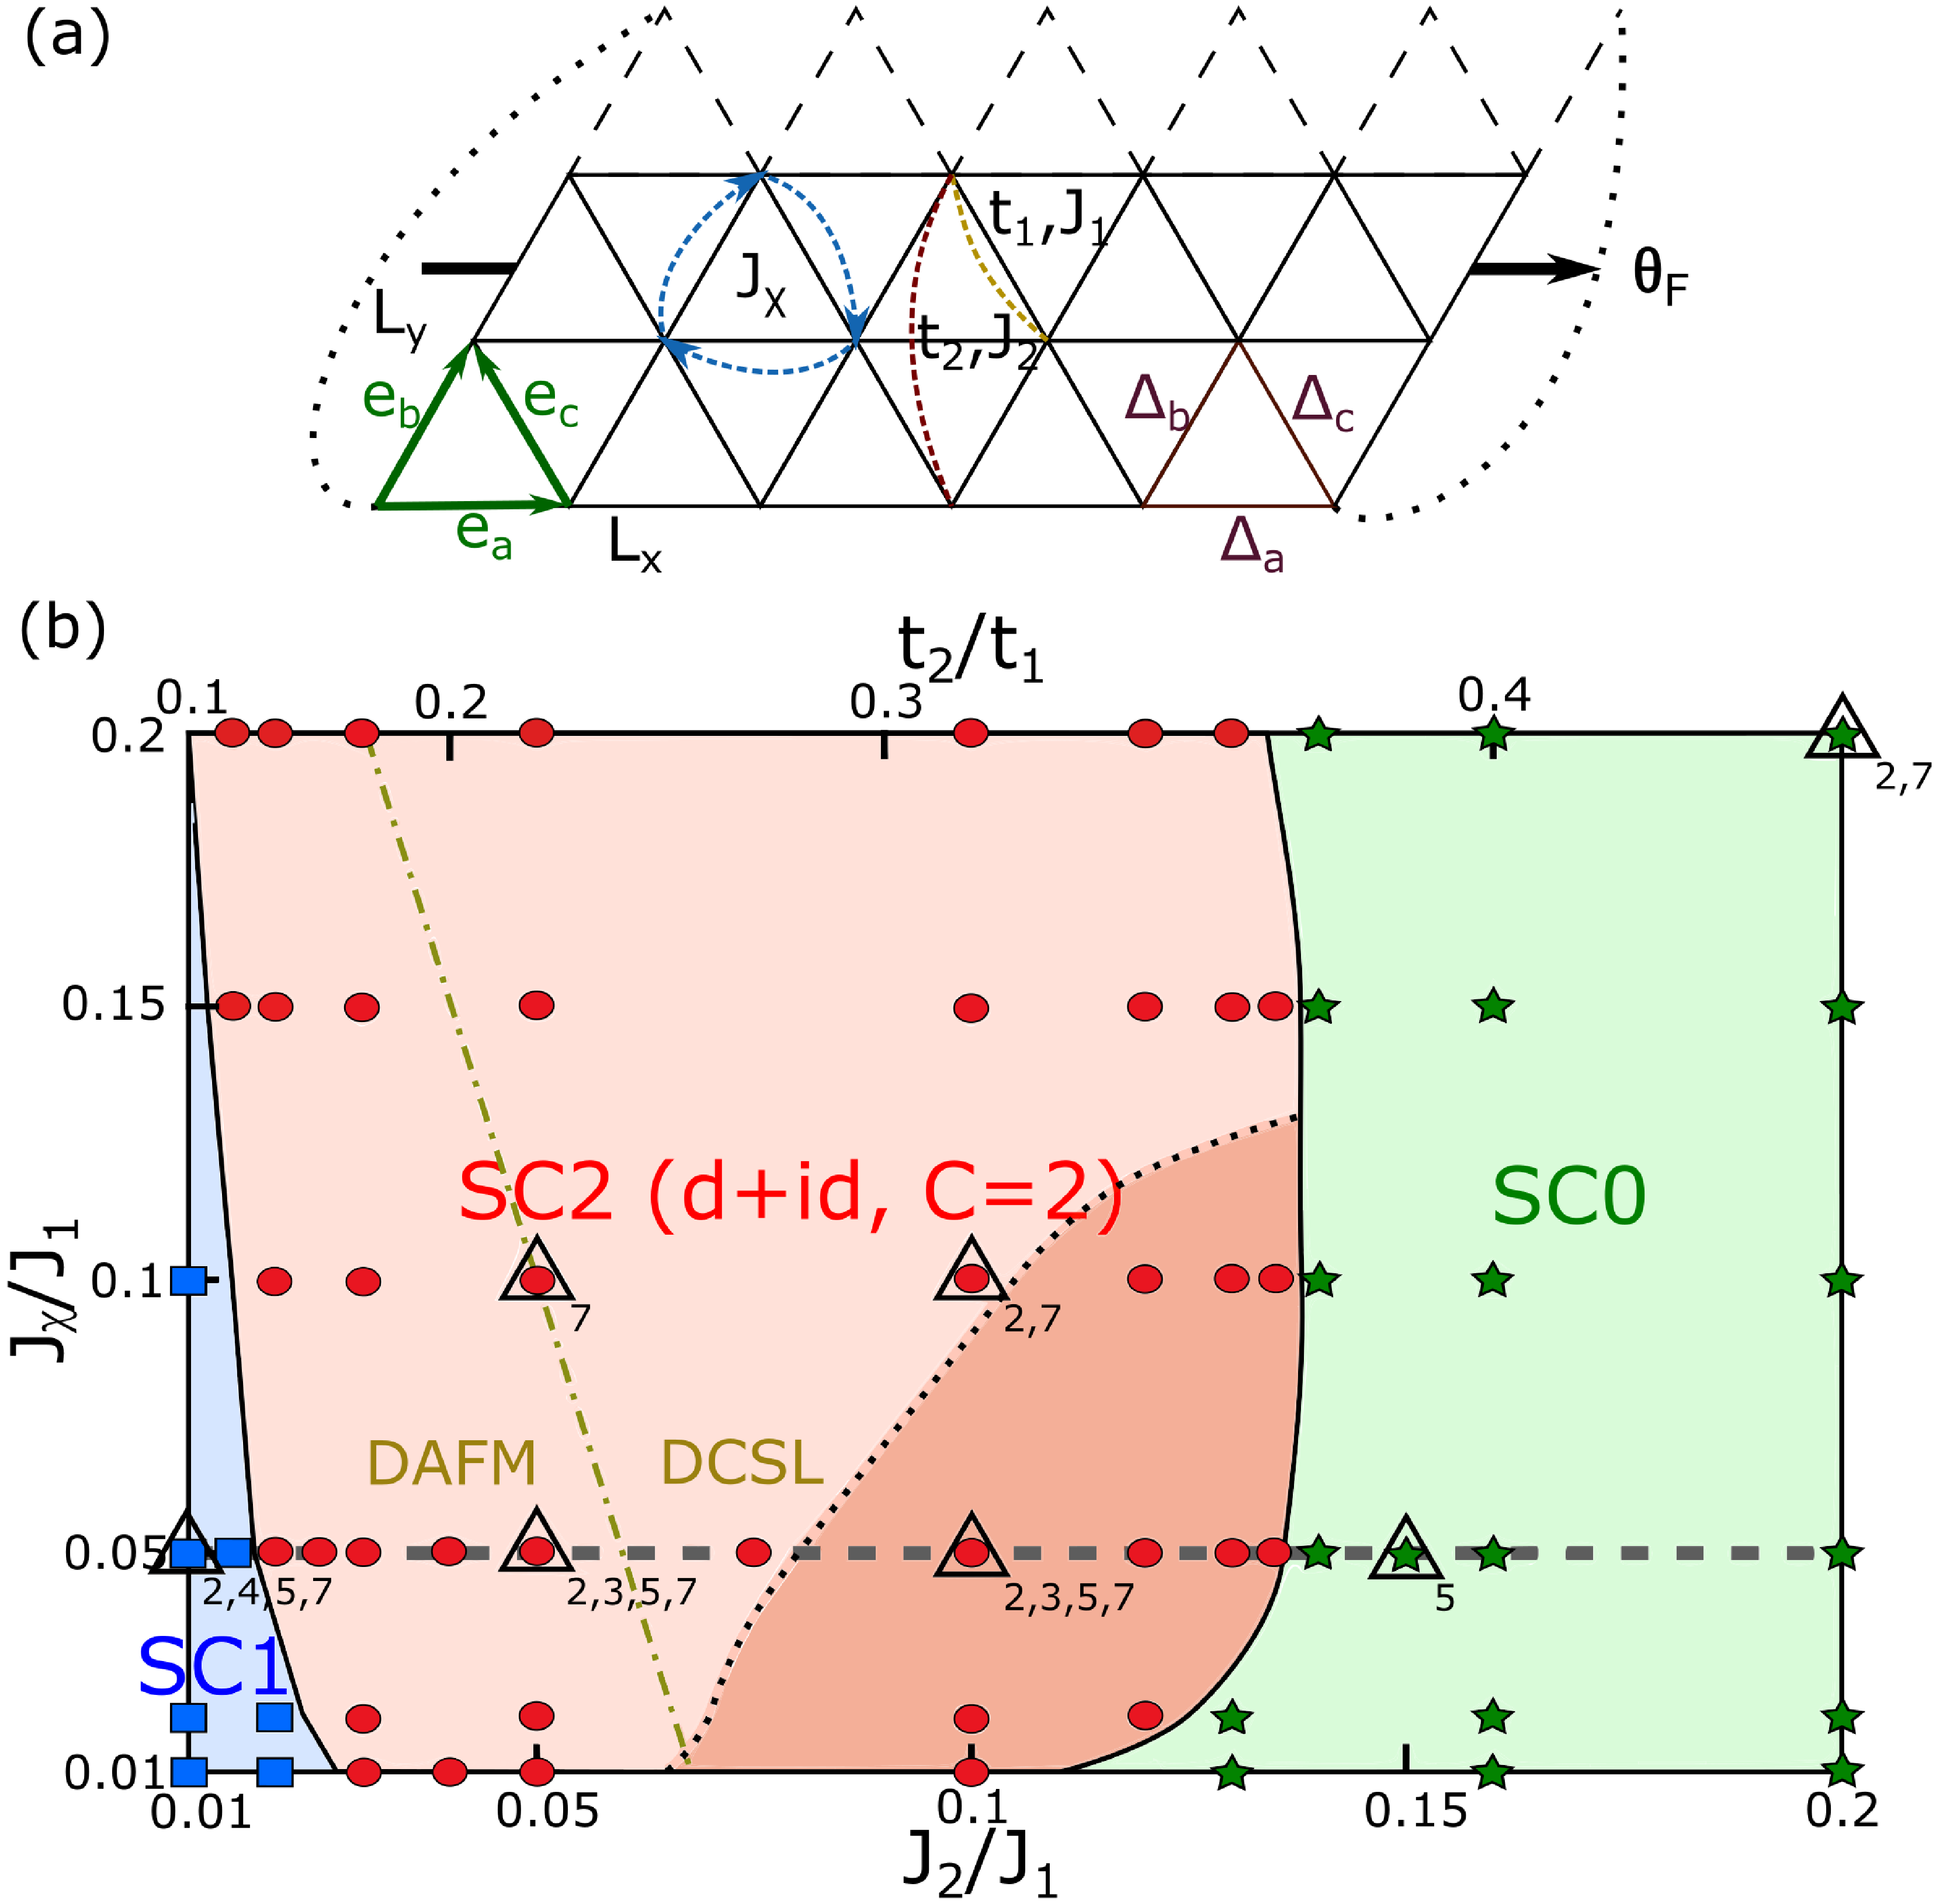
\includegraphics[width=1\linewidth]{Phase_diagram_v3.pdf}
\caption{Quantum phase diagram. (a) Schematic illustration of the extended $t$-$J$-$J_{\chi}$ model on a triangle lattice with the nearest-neighbor and the next-nearest-neighbor hoppings $t_{1}$, $t_{2}$ and Heisenberg exchange $J_{1}$,$J_{2}$ interactions, as well as the three-spin chiral interactions $J_{\chi}$. The dash lines indicate  the periodic boundary condition. (b) The quantum phase diagram obtained on  $L_{y}=6$ cylinders  based on the Chern number simulations. For  $0.01 \leq J_{2}/J_{1}, J_{\chi}/J_{1} \leq 0.2$   and doping level  $\delta=1/12$, \oim {we identify distinct classes of SC phases  labeled as SC1, SC2, and SC0 from left to right characterized  by their spin Chern number $C$. The SC2 regime represents two phases, the isotropic TSC (lighter red region) and nematic TSC  (darker red region) phases. Different symbols represent parameter points studied
with the DMRG methods.  The triangles mark  points  presented in the paper with the lower indices representing the indices of figures.  A scan of the Chern number, SC pairing symmetry and energy/entropy along the horizontal dashed line is used in Figs.~\ref{Fig_flux_insertion}(c) ,~\ref{Fig_phase_transition}(d), and~\ref{Fig_nature_transiton}, respectively. The main feature of the phase diagram is essentially the same for other doping levels $\delta=1/24-1/8$.}}
\label{Fig_phase_diagram}
\end{figure}


\begin{figure}
\centering
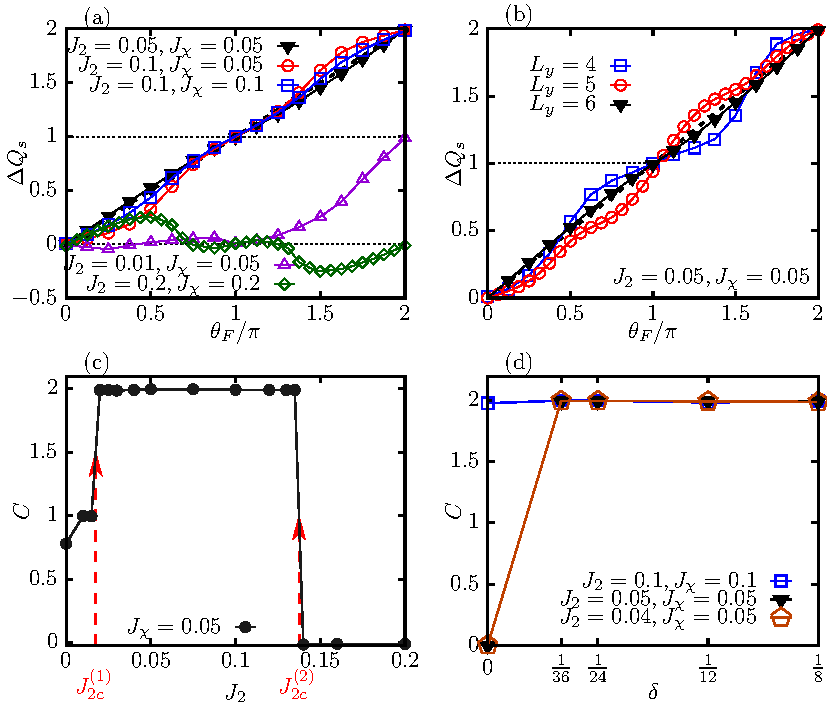
\includegraphics[width=1\linewidth]{Chern.pdf}
\caption{The pumped spin by inserting flux and spin Chern number. (a) The pumped spin $\Delta Q_{s}$ with adiabatically inserted flux $\theta_{F}$ is shown for different SC phases  on $L_{y}=6$ cylinder. For the three parameter points in the SC2 phase the measured spin pumping after inserting one flux quantum $\Delta Q_s|_0^{2\pi}=1.993, 1.983, 1.990$, respectively, indicating that the error bar is around 1\% from exactly quantized value $\Delta Q_s|_0^{2\pi}=2$ for different systems. (b) $\Delta Q_s$ versus $\theta_F$ for $J_{2}=J_{\chi}=0.05$ inside SC2 phase on $L_{y}=4, 5, 6$ cylinders. (c) The evolution of Chern number $C$ with varying $J_{2}$ at $J_{\chi }=0.05$ on $L_{y}=6$. $C=\Delta Q_s|_0^{2\pi}$ is obtained after inserting one flux quantum $\theta_F=0\rightarrow 2\pi$.  SC1-SC2 and SC2-SC0 phase transitions take place at $J_{2}=J_{2c}^{(1)},J_{2c}^{(2)}$, respectively, where  the  Chern number jumps.  The doping level is $\delta=1/12$ for (a-c). (d) $C$ versus $\delta$ for parameter points with different undoped parent states (e.g. DAFM or DCSL) on $L_{y}=6$.}
\label{Fig_flux_insertion}
\end{figure}


\section{Model and method}
\label{model_method}
We study the extended $t$-$J$-$J_{\chi}$ model that is defined as 
\begin{eqnarray}
\label{eq1}
H &=& -\sum\limits_{\left \{ ij \right \},\sigma
}t_{ij}(\widehat{c}^{\dagger }_{i,\sigma }\widehat{c}_{j,\sigma }+h.c.) + \sum\limits_{ \left \{ ij \right \} } J_{ij}(\widehat{\boldsymbol{S}}_{i}\cdot \widehat{\boldsymbol{S}}_{j}-\frac{1}{4}\widehat{n}_{i}\widehat{n}_{j})  \nonumber \\ &+& J_{\chi
}\sum\limits_{\{ ijk \} \in \bigtriangledown / \bigtriangleup  }\widehat{\boldsymbol{S}}_{i}\cdot (
\widehat{\boldsymbol{S}}_{j}\times \widehat{\boldsymbol{S}}_{k}),
\end{eqnarray} 
where $\widehat{c}_{i,\sigma}^{\dagger}$ is the electron creation operator on site $i$ with spin index $\sigma=\pm 1$, $\widehat{\boldsymbol{S}}_{i}$ is the spin-$\frac{1}{2}$ operator and  $\widehat{n}_{i}=\sum_{\sigma}\widehat{c}_{i,\sigma}^+\widehat{c}_{i,\sigma}$ is the  electron number operator.
We consider the  nearest neighbor and the next nearest neighbor hoppings $t_{1}$, $t_{2}$ as well as Heisenberg couplings $J_{1}$, $J_{2}$, supplemented by the three-spin chiral interactions $J_{\chi}$ on every elementary triangle as illustrated in Fig.~\ref{Fig_phase_diagram}(a). The chiral interaction can be generated from Hubbard model with an external magnetic field~\cite{jiang2020topological}.
We set $J_{1}=1$ as the units of energy, $t_{1}=3$, $J_{2}/J_{1}=(t_{2}/t_{1})^{2}$, and focus on the regime of $0<J_{2}, J_{\chi} \leq 0.2$ with hole doping level $\delta \leq 1/8$, which is the optimal doping region for the unconventional SC~\cite{jiang2020topological,gong2021robust}.

To obtain the ground state of the Hamiltonian in Eq.~(\ref{eq1}), we apply the  DMRG method with $U(1)\times SU(2)$ for charge and spin symmetries~\cite{McCulloch2007} on cylinder systems with open boundary condition along the axis ($e_{a}$ or $x-$) direction and periodic boundary condition along the circumferential ($e_{b}$ or $y-$)  direction, as illustrated in Fig.~\ref{Fig_phase_diagram}(a). The number of sites is $N=L_{x}\times L_{y}$ where  $L_{x}$ and $L_{y}$ denote the lengths in these two directions, respectively. 
The number of electrons $N_{e}$ is related to the doping level $N_{e}/N=1-\delta$.
We keep up to $M=12000$ SU(2) spin multiplets (equivalent to about $m=36000$ U(1) states) with  truncation error  $\epsilon \sim  10^{-6}$, which leads to  accurate results (see Supplementary Sec. ii~\cite{SuppMaterial} for details). We develop a topological characterization for the SC  states through the spin flux insertion by adiabatically evolving the ground state as a function of a twisted boundary phase $\theta_F$ based on the method established for CSL and fractional quantum Hall systems~\cite{gong2014,grushin2015characterization}. The flux adds a spin dependent phase factor to the electron hoppings $\widehat{c}_{i,\sigma}^{\dagger }\widehat{c}_{j,\sigma}\rightarrow e^{i\sigma\theta_{F}}\widehat{c}_{i,\sigma}^{\dagger}\widehat{c}_{j,\sigma}$ if $j\rightarrow i$ crossing y-boundary from the top (see Fig.~\ref{Fig_phase_diagram}(a)), and similarly couples to  the spin flip terms~\cite{gong2014}. In this type of calculations, the SU(2) symmetry is broken by the spin flux and we use $U(1)\times U(1)$ symmetries with bond dimensions up to $m=8000$ for accurate results due to the robustness of the topologically-protected spin pumping (see Supplementary Sec. i~\cite{SuppMaterial} for more details).




%%%
\section{Quantum phase diagram}
\label{phase_diagram}
At half filling (with no doping $\delta=0$), the Hamiltonian in Eq.~(\ref{eq1}) reduces to the Heisenberg $J_{1}$-$J_{2}$-$J{\chi}$ model~\cite{gong2017global}. 
In the small $J_{2}$ regime ($J_{1}=1$), the $120^{\circ}$ AFM order survives up to $J_{2}\approx 0.07$ at $J_{\chi}=0$, which
smoothly extends to the non-zero $J_{\chi}$ regime. The intermediate $J_{2}$ regime is dominated by the CSL, which separates from the AFM order by the dash dotted line as shown in Fig.~\ref{Fig_phase_diagram}(b) obtained from Ref.~\cite{ wietek2017chiral,gong2017global}. Through extensive DMRG simulations of topological Chern numbers  and SC pairing correlations on $L_{y}=4\sim 6$  cylinders for hole doped systems, we establish a quantum phase diagram in the parameter space $0<J_{2}, J_{\chi} \leq 0.2$ for doping $\delta=1/12$, with three distinct classes of superconducting phases stabilized by  small $J_{2}, J_{\chi} \geq  0.01$~\cite{note1} as shown in Fig.~\ref{Fig_phase_diagram}(b). These SC phases are characterized by  different topological spin Chern numbers. \oim{At small $J_{2}$ we find a topological chiral $d+id$-wave SC phase with spin Chern number $C = 1$ (labeled as SC1) by doping the AFM  (DAFM) state. 
In the intermediate $J_{2}$ regime, another class of topological $d+id$-wave SC phases emerges  characterized by a quantized $C = 2$ (SC2), which can be induced by doping either the AFM state or the CSL (DCSL) as illustrated in Fig.~\ref{Fig_phase_diagram}(b). 
The SC2 class is further divided into an isotropic TSC phase and a nematic TSC phase breaking rotational symmetry.
Interestingly,  the nematic TSC state is an analog state
of the recently revealed nematic fractional quantum Hall effect~\cite{haldane2011geometrical,you2014theory, yang2017anisotropic,regnault2017evidence}. 
At larger $J_{2}$, the SC phase has a d-wave symmetry with anisotropic pairing correlations  breaking the lattice rotational symmetry and $C=0$ (SC0) indicating a topologically-trivial SC phase.  The SC0 phase  belongs to the same quantum phase as the nematic d-wave SC identified for an extended $t$-$J$ model~\cite{jiang2021superconductivity} with time-reversal symmetry.} The phase  diagram is essentially the same for other doping levels $\delta=1/24-1/8$ with small shifts in phase boundaries (e.g. at $\delta=1/8$,  $\Delta J_{2c}^{(1)}\approx  0.01\sim 0.02$ where $J_{2c}^{(1)}$ denotes the critical $J_{2}$ between SC1 and SC2). We also find that the previously revealed $d+id$-wave SC state (at $J_{\chi}=0.4$ and $J_{2}=t_{2}=0.0$)~\cite{jiang2020topological} has $C=2$ sitting near the phase boundary of SC2  phase.
%%%
\subsection{Topological Chern number characterization  through flux insertion}
\label{flux_insertion}
The nonzero  Chern number characterizes the topological nature of the $d+id$-wave superconductors~\cite{read2000paired,senthil1999spin}, which also identifies the number of the chiral Majorana edge modes. 
We determine  the spin Chern number through the spin pumping with inserting flux $\theta _{F}$ into the cylinder, as illustrated in Fig.~\ref{Fig_phase_diagram}(a).  The net spin with nonzero $S_z$ accumulates near the boundaries of the cylinder as the flux adiabatically increases, while the total $S_{z}=0$ for the ground state at different $\theta_F$. We use a small step for the increase of the flux $\theta_F \rightarrow \theta_F+\Delta \theta_F$ with $\Delta \theta_F=2\pi/16$.
A finite Chern number~\cite{gong2014} can be obtained from the total spin  pumping $C=\Delta Q_{s}|_0^{2\pi}= (n_{\uparrow}-n_{\downarrow})|_0^{2\pi}$  measured at left boundary  at $\theta _{F}=0$ and $2\pi$, where $n_{\sigma}$ is the accumulated charge near the boundary with spin $\sigma$.  We directly measure the pumped spin  for each $\theta_F$ from the reduce density matrix by calculating the sum $Q_{s}=\sum_{\alpha}\lambda _{\alpha}(n_{\uparrow,\alpha}-n_{\downarrow,\alpha})$, where  $\lambda _ {\alpha }$ is the eigenvalue  and $\alpha$ the eigenstate of the reduced density matrix~\cite{grushin2015characterization}, and  $n_{\uparrow,\alpha}$ ($n_{\downarrow,\alpha}$) is the particle number of the  $\alpha$ state with up (down) spin. Because the inserted flux breaks SU(2) symmetry, we use infinite DMRG with $U(1)\times U(1)$ symmetries with a large unit cell that is commensurate with the doping level (see Supplementary Sec. i~\cite{SuppMaterial}). 

\begin{figure}
\centering
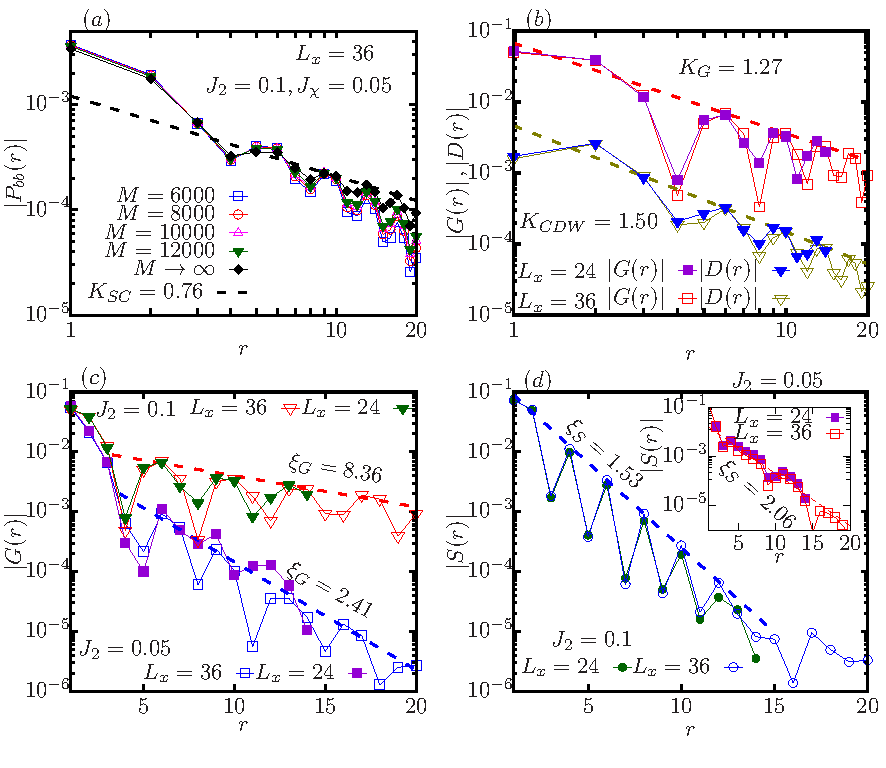
\includegraphics[width=1\linewidth]{SC_density_correlation_fit_new.pdf}
\caption{Pairing and other correlations in SC2. (a) The SC pairing correlations for different  bond dimensions $M$ at $J_{2}=0.1,J_{\chi}=0.05$ for $N=36\times 6$ system. $\mathbf{r}$ is chosen along x-direction $\mathbf{r}=(r,0)$ and the reference point is $\mathbf{r}_{0}=(L_{x}/4,y_{0})$ to avoid the boundary effect (the results are independent of $y_{0}$ because of the translational invariant along y-direction). The  straight-line fit in the log-log plot of the extrapolated data in the infinite $M$ limit follows a power-law behavior. (b) The density-density correlation $\left |D(r)\right |$ and single particle correlation $\left |G(r)\right |$ which are fit by the power-law relation for $N=24\times 6$ and $36\times 6$, at $J_{2}=0.1,J_{\chi}=0.05$.
(c) The comparison of $\left |G(r)\right |$ at $J_{2}=0.05$ and $0.1$ with  the same $J_{\chi}=0.05$, which demonstrates the fast growing of the correlation length $\xi_G$ with the increase of $J_{2}$. (d) The exponential decay of the spin correlations $\left |S(r)\right |$ in the main figure and its inset for the same parameters as in (c), where $r > 15$ data points are  ignored in the fitting  because their values are comparable to the numerical truncation error. \oim{The doping level is $\delta=1/12$. The obtained fitting exponents or correlation lengths have error bars around 0.02, except for the one in the inset of (d) which is around 0.06.}}
\label{Fig_SC_correlation}
\end{figure}

We show examples of the flux insertion and the resulting Chern numbers for systems with $\delta=1/12$ in Fig.~\ref{Fig_flux_insertion}(a). For three parameter points inside the SC2 phase on $L_{y}=6$ system, the $\Delta Q_{s}$ increases almost linearly with $\theta _{F}$ indicating uniform Berry curvature~\cite{sheng2006}, and there is $\Delta Q_{s}\approx 2.0$ net spin  pumped to  the boundary after the threading of one flux quantum ($\theta_F=0\rightarrow 2\pi$). This corresponds to the quantized Chern number $C=2$, which remains the same on various $L_{y}=4$, $5$, and $6$ as shown in Fig.~\ref{Fig_flux_insertion}(b). The pumping rate becomes more uniform with the increase of $L_{y}$, indicating the increased robustness of the topological quantization for larger systems.   In contrast, at $J_{2}=0.01,J_{\chi}=0.05$ inside the SC1 phase, we find no linear relation between $\Delta Q_{s}$ and $\theta _{F}$ which indicates the nonuniform Berry curvature versus boundary phase $\theta_F$~\cite{sheng2006}. The measured $\Delta Q_{s}\approx 0.983$, indicating around one  net spin  pumped  with the insertion of one flux quantum and $C = 1$. The Chern number becomes non-quantized extended to the $J_{2}=0$ limit  as shown in Fig.~\ref{Fig_flux_insertion}(c) signaling gapless low energy excitations. We believe the large  variance of the Berry curvature versus $\theta_F$ for SC1 phase may indicate a  topological state with gapless excitations at small $J_{2}$ consistent with an early proposal for
topological superconducting state for Na$_x$CoO$_2$·yH$_2$O system based on variational simulations~\cite{zhou2008nodal}. In the SC0 phase at larger $J_{2}=J_{\chi }=0.2$, we find $\Delta Q_{s}\approx -0.01$ which confirms $C = 0$ for a topologically-trivial SC state. Thus, the phase transitions between the three phases can be characterized by jumps of topological Chern number $C$ with varying $J_{2}$ at a fixed $J_{\chi}=0.05$ as illustrated in Fig.~\ref{Fig_flux_insertion}(c). 

Since the undoped $(\delta=0)$ parent state of the SC2 phase contains both the AFM state and  CSL, a natural question is how the Chern number evolves with the doping level. As demonstrated in Fig.~\ref{Fig_flux_insertion}(d), for two points in the DAFM regime at $J_{2}=0.04,0.05$ and $J_{\chi}=0.05$, $C$ jumps from 0 to 2 at  a small doping of $\delta=1/36$ and remains quantized at $C=2$ for larger $\delta$, which demonstrates a doping induced topological quantum phase transition. On the contrary, in the DCSL regime at $J_{2}=J_{\chi}=0.1$, $C=2$ for $\delta=0-1/8$ which shows a robust Chern number quantization from the parent CSL to the topological $d+id$-wave SC. This is consistent with the fact that the KL-CSL is a bosonic $\nu =1/2$  fractional quantum Hall  state~\cite{kalmeyer1987equivalence,wen1989chiral,read2000paired}, which is equivalent to the $C=2$ topological order for fermionic systems where the phase space is enlarged by a factor 4 in the definition of Chern number~\cite{hu2015variational} with a doubled flux period  for the Hamiltonian to be invariant. The exact quantization $C=2$ of the SC2 phase indicates that doped holes can indeed adjust the internal flux with the hole doping level to realize bosonic integer quantum Hall effect for holons~\cite{song2021doping}. 

%%%
\subsection{Quasi-long-range order in superconducting pairing correlations}
\label{SC_correlation}
To explore the superconducting nature of the system,  we focus on  the dominant spin singlet pairing correlations $P_{\alpha \beta }(\mathbf{r})=<\widehat{\Delta} ^{\dagger }_{\alpha }(\mathbf{r}_{0})\widehat{\Delta} _{\beta }(\mathbf{r}_{0}+\mathbf{r})>$, where the pairing operator $\widehat{\Delta} _{\alpha }(\mathbf{r})=(\widehat{c}_{\mathbf{r}\uparrow}\widehat{c}_{\mathbf{r}+e_{\alpha }\downarrow}-\widehat{c}_{\mathbf{r}\downarrow}\widehat{c}_{\mathbf{r}+e_{\alpha }\uparrow})/\sqrt{2}$  with $\alpha = a,b,c$, representing different nearest neighboring bonds as illustrated in Fig.~\ref{Fig_phase_diagram}(a). 

\begin{figure}
\centering
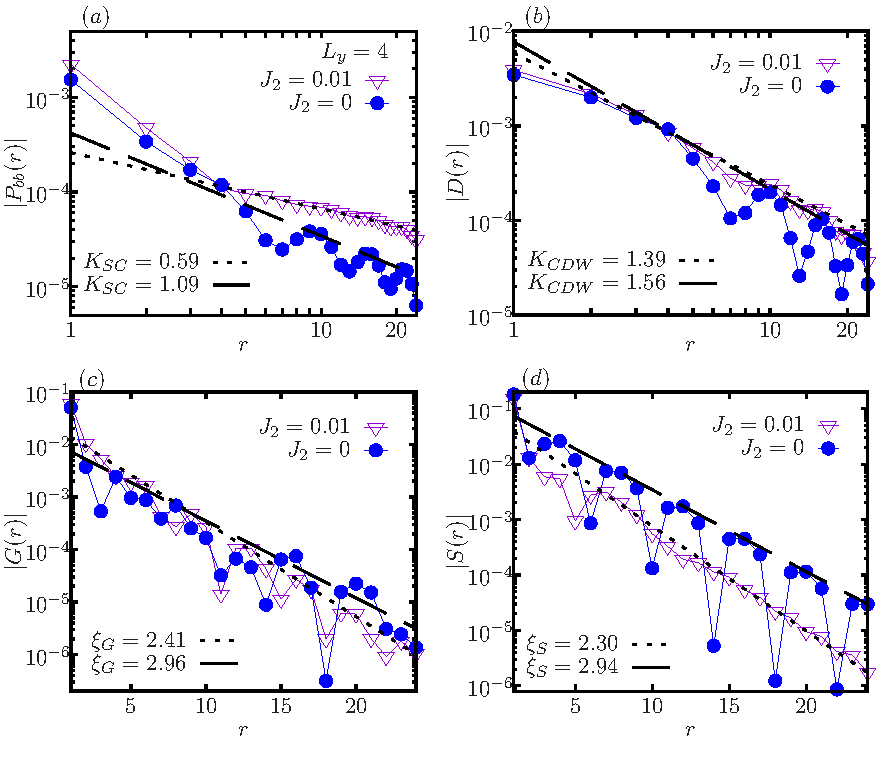
\includegraphics[width=1\linewidth]{SC_density_correlation_SC1.pdf}
\caption{\oim{Pairing and other correlations at $J_{\chi}=0.05$ for smaller $J_{2}$ on $L_{y}=4$. The results are converged with a large bond dimension $M=10000$. (a) The SC pairing correlations. $\mathbf{r}$ is chosen along x-direction $\mathbf{r}=(r,0)$ and the reference point is $\mathbf{r}_{0}=(L_{x}/4,L_{y}/2)$ to avoid the boundary effect. The straight-line fit in the log-log plot follows a power-law behavior, with  exponents of $1.09$ and $0.59$ for $J_{2}=0$ and $0.01$, respectively. (b) The density-density correlations $\left |D(r)\right |$ which are fit by a power-law relation, with  exponents of $1.56$ and $1.39$ for $J_{2}=0$ and $0.01$, respectively. (c) The single particle correlations $\left |G(r)\right |$ which are fit by an exponential decay with  correlation lengths of $2.96$ and $2.41$ for $J_{2}=0$ and $0.01$, respectively. (d) The spin correlations $\left |S(r)\right |$ which are fit by an exponential decay with  correlation lengths of $2.94$ and $2.30$ for $J_{2}=0$ and $0.01$, respectively. The doping level is $\delta=1/12$. The obtained fitting exponents or correlation lengths have  error bars around 0.03.}}
\label{Fig_SC1}
\end{figure}

We first give an example of  the SC pairing correlations in the SC2 regime as shown in Fig.~\ref{Fig_SC_correlation}(a), where the magnitude of pairing correlations at longer distance for two b-bonds (along $y$-direction) $\left | P_{bb}(r) \right |$  increases gradually as the DMRG bond dimension increases from $M=6000$ to $12000$ at $J_{2}=0.1,J_{\chi}=0.05$ on $N=36\times 6$ system.
Because DMRG represents the ground state in the matrix product form~\cite{schollwock2011density} with finite bond dimensions, the scaling to $M\rightarrow \infty$ is needed to identify the true nature of long-distance correlations for wider cylinders. 
Using a second-order polynomial fitting of $1/M$, we find that the extrapolated $\left | P_{bb}(r) \right |$ shows a power-law decay with distance  $\left | P_{bb}(r) \right |\sim r^{-K_{SC}}$, with the Luttinger exponent $K_{SC}\approx 0.76$. Similar results are obtained for correlations with other bonds, and also for different $L_{x}$ or  $L_{y}=4$  systems (see Supplementary Sec. iii. A~\cite{SuppMaterial}). The  $K_{SC}\lesssim 1$ holds for SC2 phase, indicating a strong divergent SC susceptibility in the zero-temperature limit~\cite{jiang2021superconductivity}.

We then turn to the density-density  $D(\mathbf{r})=<\widehat{n}_{\mathbf{r}_{0}} \widehat{n}_{\mathbf{r}_{0}+ \mathbf{r}}>-<\widehat{n}_{\mathbf{r}_{0}}><\widehat{n}_{\mathbf{r}_{0}+ \mathbf{r}} >$ and single particle $G(\mathbf{r})=\sum _{\sigma }< \widehat{c}^{\dagger }_{\mathbf{r}_{0},\sigma } \widehat{c}_{\mathbf{r}_{0}+\mathbf{r},\sigma }>$ correlations. As shown in Fig.~\ref{Fig_SC_correlation}(b), the $\left |D(r) \right |$ decays with a power-law relation at long distance  using extrapolated data. The Luttinger exponent for density-density correlations is $K_{CDW}\approx 1.50$ much larger than $K_{SC}$. %  is larger for wider $L_{y}$ systems while  $K_{SC}$ becomes smaller, 
%%The  $K_{SC}K_{CDW}\approx 1.14\approx 1$ is consistent with the Luther-Emery liquid~\cite{luther1974backward}.
Both   $\left | P_{bb}(r) \right |$  and  $\left |D(r) \right |$ show similar spatial oscillations consistent with the  electron  density  oscillation  in  real  space (see Supplementary Sec. v~\cite{SuppMaterial}).
Similarly, the single particle Green function $\left |G(r)\right |$ can also be fit into power-law behavior  (Fig.~\ref{Fig_SC_correlation}(b)).
Interestingly, we identify a crossover for $\left |G(r)\right |$ with the increase of $J_{2}$. At smaller $J_{2}=0.05$ in the SC2 regime, we observe an exponential decay in $\left |G(r)\right |$ with a short correlation length $\xi_G\approx 2.41$ which is consistent with the gapped isotropic TSC state as shown in Fig.~\ref{Fig_SC_correlation}(c). With the increase of $J_{2}$, the correlation length for $\left |G(r)\right |$ increases to $\xi_G\approx 8.36$ larger than $L_{y}$, which could also be fitted by a power-law decay (as shown in Fig.~\ref{Fig_SC_correlation}(b)) at $J_{2}=0.1$ for fixed  $J_{\chi}=0.05$ on different systems $N=24\times6$ and $36\times 6$.
The evolution of the single particle correlation length is a signature of the evolution of the quasi-particle excitation gap, which gradually reduces
with the increase of the $J_{2}$ approaching the quantum phase transition \oim{ from gapped SC state to a nodal nematic SC state as we will address further in Sec.~\ref{symmetry_evolutions}.}
In comparison, the spin-spin correlations remain exponentially decay with a short correlation length $\xi _{S}\approx 1.53$  ($2.06$) as shown in the main panel (inset) of Fig.~\ref{Fig_SC_correlation}(d) at $J_{2}=0.1$ ($0.05$), indicating a finite spin gap which protects the SC state. \oim{
These results provide compelling evidence for the robust SC pairing correlations as dominant correlations for SC phases
with $C=2$, which are  the quasi-1D descendent states of  2D topological superconductors.

Now we  discuss the  features of various correlations at small $J_{2}$, where the SC1 phase is identified with the Chern number $C=1$.
The SC pairing correlations are shown in Fig.~\ref{Fig_SC1}(a), where the magnitude of the SC pairing correlations  $\left | P_{bb}(r) \right |$ show power-law behavior with the Luttinger exponents $K_{SC}\approx 1.09$ and $0.59$ for $J_{2}=0$ and $0.01$, respectively, obtained with a fixed $J_{\chi}=0.05$ for $N=48\times 4$ system.
In comparison,  as shown in Fig.~\ref{Fig_SC1}(b), the $\left |D(r) \right |$ decays with a power-law relation with larger exponents ($K_{CDW}\approx 1.56$ and $1.39$),
while the  $\left |G(r)\right |$ (Fig.~\ref{Fig_SC1}(c)) and  $|S(r)|$ (Fig.~\ref{Fig_SC1}(d)) both decay exponentially with small correlation lengths.
These results indicate that SC1 phase has dominant SC correlations observed for $L_{y}=4$ cylinders.
We also confirm  power-law SC correlations for a wider system of $N=20\times 6$ at $J_{2}=0.01, J_{\chi }=0.05$ with good numerical convergence for this possible gapless phase.  
Interestingly, there are stronger spin correlations for the $L_{y}=6$ system indicating a vanishing or very small spin gap
(see Supplementary Sec. iii. D~\cite{SuppMaterial}), which is consistent with the fact that the SC1 phase has a spin gap-closing transition from $C=2$ phase.

 

We further confirm that the SC0 phase has robust quasi-long-range SC pairing correlations with a Luttinger exponent $K_{SC}\approx 1.10$ at $J_{2}=J_{\chi}=0.2$ dominating the density-density correlations. This phase can be smoothly connected to the d-wave phase identified by doping the $J_{1}$-$J_{2}$ model~\cite{jiang2021superconductivity} with lager $J_{2}$ (see Supplementary Sec. iii. C~\cite{SuppMaterial} for more details).
%Other parameters marked with the triangles in Fig.~\ref{Fig_phase_diagram}(b) are also tested to give similar dominant SC %pairing correlations.

There are other competing quantum phases and additional quantum phase transitions 
as we reduce the three spin chiral interactions to zero in the small $J_{2}$ regime. For example, at $J_{2}=J_{\chi }=0$, 
the ground state is dominated by charge stripe and spin fluctuations with suppressed pairing correlations.
Furthermore,  additional results for $L_{y}=4$ with small $J_{2}$ for a possible pairing density wave SC phase~\cite{peng2021gapless}, and a d-wave SC phase co-existing with phase separation are shown in the Supplementary Sec. iii. F~\cite{SuppMaterial}.
These results provide further support that a small but finite chiral interaction plays an important role in stabilizing the topological SC phases for the systems we have studied.   }


%%%
\subsection{Pairing symmetry for topological and nematic SC phases}
\label{pairing_symmetry}
The SC pairing symmetry can be identified by the phases of the pairing correlations for different bonds.
To extract the phase we rewrite the SC pairing correlation as $P_{\alpha \beta }(\mathbf{r})=\left | P_{\alpha \beta }(\mathbf{r}) \right |e^{i\phi _{\alpha \beta }(\mathbf{r})}$ where $\phi _{\alpha \beta }(\mathbf{r})$ is the phase for the correlation, and  the pairing order parameter as $\Delta_{\alpha}(\mathbf{r})=\left | \Delta_{\alpha}(\mathbf{r}) \right |e^{i\theta _{\alpha}(\mathbf{r})}$.  Using the definition of the pairing correlations, we obtain $\theta_{\alpha\beta}(\mathbf{r})=\theta_{\alpha}(\mathbf{r})-\theta_{\beta}(\mathbf{r})=\phi_{\alpha\alpha}(\mathbf{r})-\phi_{\alpha\beta}(\mathbf{r})$
as the relative phases of the pairing order parameters  for different nearest neighbor bonds; see illustrations in the inset of Fig.~\ref{Fig_phase_transition}(a). The  pairing symmetry for  different SC states are illustrated in Fig.~\ref{Fig_phase_transition}(a) on $N=36\times6$ systems. At $J_{2}=J_{\chi}=0.05$ in the SC2 regime,  $\theta _{\alpha \beta }(r)$ remains almost independent of $r$ and the phases for order parameters are nearly quantized to $[{\theta }_{bb },{\theta }_{bc},{\theta }_{ba}]\approx [0,-0.64\pi, 0.65\pi] \approx [0,-\frac{2}{3}\pi,\frac{2}{3}\pi]$, which represents an isotropic $d+id$-wave  with $C_3$ rotational symmetry. The angles ${\theta }_{ba},{\theta }_{bc}$ are closer to $\pm 2\pi/3$ on wider system $L_{y}=6$  compared with $L_{y}=4$ results (with $L_{x}=48$) as shown in  Figs.~\ref{Fig_phase_transition}(a) and (b). At larger $J_{2}=0.15$ with $J_{\chi}=0.05$ in the SC0 phase, these phases become $[{\theta }_{bb },{\theta }_{bc },{\theta }_{ba }]\approx [0,-0.93\pi, 0.93\pi]\approx [0,-\pi, \pi]$, which are nearly independent of  $L_{y}=4$ or $6$, suggesting  a d-wave SC state consistent with the Chern number $C=0$ for this phase. 


\begin{figure}
\centering
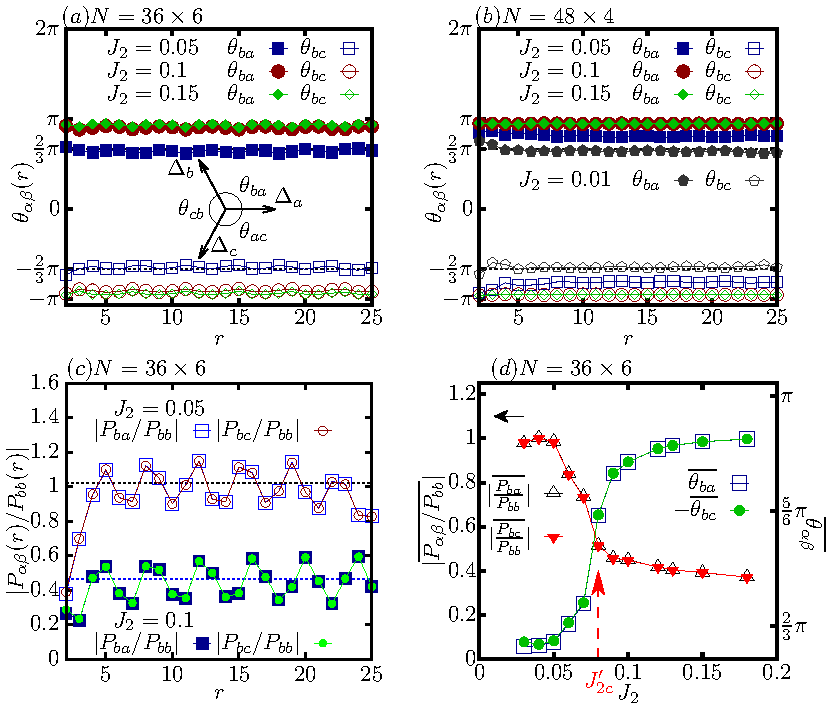
\includegraphics[width=1\linewidth]{Phase_transition_v4.pdf}
\caption{Transition from the $d+id$-wave SC2 phases to SC0 phase. (a) The spacial dependence of relative phases for SC  order parameters for various $J_{2}$ on $L_{y}=6$ ($L_{x}=36$) system. $\mathbf{r}$ is chosen along x-direction $\mathbf{r}=(r,0)$.  (b) The relative phases for SC order parameters on $L_{y}=4$ ($L_{x}=48$) system.  (c) The ratio of the magnitudes of different SC  correlations. The dash line indicates the average over distances. (d) The spatial average values of the relative phases of SC order parameters and the ratios of  magnitudes of different SC correlations for various $J_{2}$. All results are obtained at $J_{\chi }=0.05$ with bond dimension $M=10000$ ($M=8000$) on $L_{y}=6$ ($L_{y}=4$) systems. The doping level is $\delta=1/12$.}
\label{Fig_phase_transition}
\end{figure}

On the other hand,  the relative strength of the SC correlations for different bonds also evolves with the increase of $J_{2}$. As shown in Fig.~\ref{Fig_phase_transition}(c), $|P_{ba}(r)/P_{bb}(r)|$ and $|P_{bc}(r)/P_{bb}(r)|$ have spatial oscillations, and  remain almost a constant average as $r$ increases, which suggests a power-law decaying behavior of $\left | P_{ba}(r) \right |$ and $\left | P_{bc}(r) \right |$ with the same exponents  $K_{SC}$. At smaller $J_{2}=0.05$, the ratios $|P_{ba}(r)/P_{bb}(r)|$ and $|P_{bc}(r)/P_{bb}(r)|$ are close to $1.0$, while they drop to around $0.46$  observed at $J_{2}=0.1$, keeping the same $J_{\chi}=0.05$.
 We further show an example of the SC1 phase at  $J_{2}=0.01$  and $J_{\chi}=0.05$ on $L_{y}=4$ in Fig.~\ref{Fig_phase_transition}(b) with nearly quantized phases $[{\theta }_{bb },{\theta }_{bc},{\theta }_{ba}]\approx [0,-0.64\pi, 0.64\pi]\approx [0,-\frac{2}{3}\pi,\frac{2}{3}\pi]$.   From mean-field theory, the isotropic SC1 state with $C=1$ has nodal quasi-particle excitations~\cite{zhou2008nodal} and   we leave the full nature of this state to the future study due to the increased  difficulty of  converging the SC correlations for this critical phase on $L_{y}=6$.


\section{Symmetry evolution and phase transitions}
\label{symmetry_evolutions}

 \subsection{Evolution of the pairing order parameters}
 \label{pairing_order_evolution}
 
 \oim{Now we focus on the symmetry evolution of the pairing order parameters from SC2 phases to SC0 phase.
 As shown in Fig.~\ref{Fig_phase_transition}(d), the $-\overline{\theta _{bc }}$ and $\overline{\theta _{ba}}$
 averaged over the middle $24$ columns of the system with $L_{x}=36$
 increase monotonically from $\frac{2}{3}\pi $ towards $\pi$ as $J_{2}$ increases.
At the same time,  we find direct evidence of the increased nematicity as $J_{2}$  increases, which is identified by the ratio of the 
 magnitudes of SC pairing correlations  for different bonds. As shown in Fig.~\ref{Fig_phase_transition}(d), the spatial averaged ratios  $\overline{ \left |P_{ba} / P_{bb} \right| }$ and $ \overline{ \left |{P}_{bc} / {P}_{bb} \right |}$ decrease monotonically from 1 to around 0.4 at larger $J_{2}$  side.
 A transition from an isotropic TSC phase to a nematic SC phase takes place inside the SC2 regime as indicated by the arrow in  Fig.~\ref{Fig_phase_transition}(d) pointing to a critical $J_{2c}'$, where both the 
$\overline{ \left |P_{ba} / P_{bb} \right| }$ and $ \overline{ \left |{P}_{bc} / {P}_{bb} \right |}$
decrease quickly to the near saturated value. This feature revealed by the nematicity evolution shows a transition inside the SC2 regime, indicating that a nematic TSC phase emerges for $J_{2c}' < J_{2} <J_{2c}^{(2)}$.
 %indicating a transition to the extended d-wave SC state~\cite{jiang2021superconductivity} where the winding of the %pairing order parameter becomes zero as extrapolated from the zero Chern number. 
As shown in Fig.~\ref{Fig_phase_diagram}(b), we identify a finite regime with increased nematicity in the SC pairing correlations while its topological nature remains the same with the Chern number $C=2$, which is consistent with  a nematic TSC state emerging within $C=2$ class of SC phases. The phase boundary is determined by the quick increase of $\overline{\theta _{ba}}$ to around $\frac{5}{6}\pi$. The emergent nematic TSC state is an analog state to the nematic fractional quantum Hall state with gapless collective excitations~\cite{haldane2011geometrical,you2014theory,yang2017anisotropic,regnault2017evidence}.} With further increase of $J_{2}$, the topological quantum phase transition takes place where the nematic d-wave SC state is recovered in  the SC0 phase.

\subsection{Nature of quantum phase transitions}
\label{phase_transition}
 
\oim{We now explore the nature of quantum phase transitions by following the energy and entanglement entropy evolution along the parameter line of $J_{\chi}=0.05$. To  calculate the entanglement entropy $S$, the cylinder is cut into two equal halves and $S$ is  obtained  from the eigenvalues $\lambda_i$ of the reduced density matrix $S =-\sum _{i} \lambda_{i}log (\lambda _{i})$.
As shown in Fig.~\ref{Fig_nature_transiton}(a), the energy per site $E_0$ shows 
a small kink and the entropy $S$ shows a large jump at $J_{2c}^{(1)}\approx 0.021$ which is very close to the transition point between $C=1$ and $C=2$ phase, indicating a first order transition between SC1 and the isotropic TSC (SC2) phase. The first order transition is further revealed by $-dE_{0}/dJ_{2}$ given in Fig.~\ref{Fig_nature_transiton}(b), which shows discontinuity around $J_{2c}^{(1)}$. Two other transitions from the isotropic TSC to nematic TSC and from nematic TSC to d-wave SC are continuous transitions with smooth evolution of $E_{0}$ and $S$ (Fig.~\ref{Fig_nature_transiton}(a)), and their derivatives (Figs.~\ref{Fig_nature_transiton}(c) - (f)). Interestingly, the transition point between the isotropic TSC to nematic TSC is indicated by the peak in $-dS/dJ_{2}$, which is very close to the one identified by the nematicity in SC pairing correlations. The transition between nematic TSC and the nematic d-wave SC may be identified by the peak in $d^{2}S/dJ_{2}^{2}$, which is shifted from the one identified by the Chern number with flux insertion into a very long cylinder studied in the infinite DMRG.  This may be explained by
the finite size effect  for identifying higher order transitions where the peaks in entropy  usually shift with system lengths~\cite{zhong2009quantum,zhang2021fidelity}. }
 
 \begin{figure}
\centering
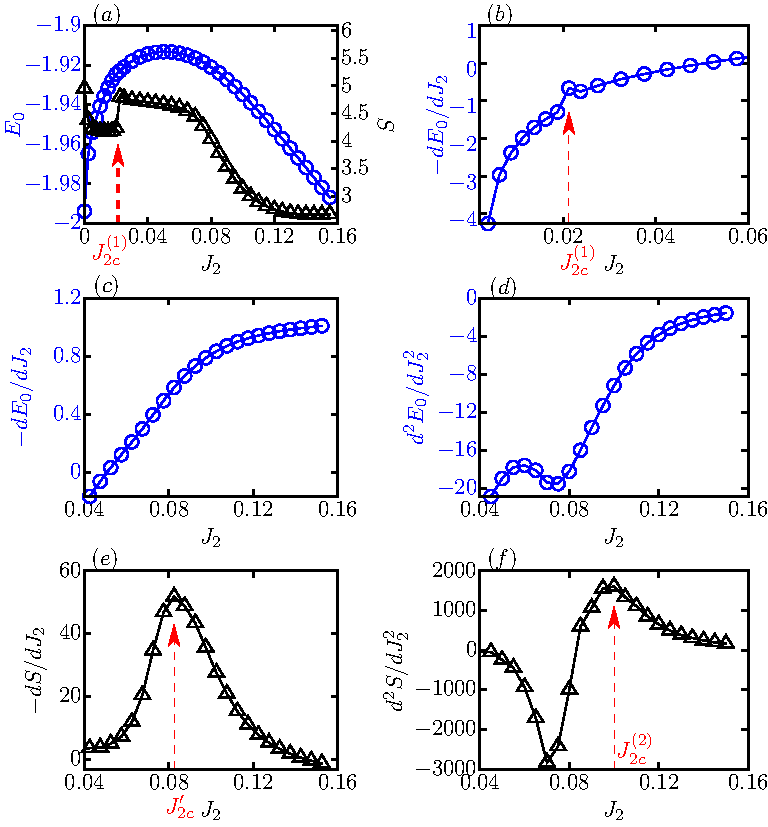
\includegraphics[width=1\linewidth]{Nature_Phase_tranistion.pdf}
\caption{\oim{The energy per site $E_{0}$ and entanglement entropy $S$ for various $J_{2}$ obtained at fixed $J_{\chi }=0.05$ on a $N=16\times 6$ cylinder. (a) The energy and entanglement entropy, where $J_{2c}^{(1)}$ is identified from  the small jump in $S$. 
(b) The first order derivative of $E_{0}$ with respect to $J_{2}$ where $J_{2c}^{(1)}$ is  identified at the discontinuity point. (c) The first order derivative of $E_{0}$ for larger $J_{2}$. (d) The second order derivative of $E_{0}$ for larger $J_{2}$. (e) The first order derivative of $S$ where $J_{2c}'$ is identified as the peak. (f) The second order derivative of $S$ where $J_{2c}^{(2)}$ is identified as the peak. The results are obtained with $M=10000$. The doping level is $\delta=1/12$.}}
\label{Fig_nature_transiton}
\end{figure}
 

\subsection{Evolution of the spin correlations}
 \label{spin_correlations}
The evolution of spin correlations can be studied through the spin structure factor defined as   $S(\mathbf{k})$ $=\frac{1}{N^{'}}\sum_{i,j}\left \langle \mathbf{S}_{i} \cdot \mathbf{S}_{j} \right \rangle e^{i\mathbf{k}\cdot (\mathbf{r}_{i}-\mathbf{r}_{j})}$ for a system with $N=36\times 6$, where $i$, $j$ are summed over the middle $N^{'}=2L_{y} \times L_{y}$ sites to avoid boundary effects. As shown in Fig.~\ref{Fig_spin_structure}(a),  $S(\mathbf{k})$ has strong peaks at the $\mathbf{K}$ points representing strong $120^{\circ}$ AFM fluctuations at short distances for $J_{2}=0.01,J_{\chi}=0.05$ inside SC1 phase, while the spin correlations exponentially decay at long distance for \oim{ all three classes of SC phases }(see Supplementary Sec. iii. E~\cite{SuppMaterial} for details). With a larger $J_{2}=0.05$ in the SC2 phase, $S(\mathbf{k})$ becomes nearly featureless with some intensity around the Brillouin zone boundaries as shown in Figs.~\ref{Fig_spin_structure}(b) and (c), which is consistent with an isotropic $d+id$-wave TSC state. As $J_{2}$ further increases to $0.1$, moderate peaks appear in $S(\mathbf{k})$ at the $\mathbf{M}$ points with nematicity as seen in Figs.~\ref{Fig_spin_structure}(d) and (e), where the SC pairing order parameters also become anisotropic (Fig.~\ref{Fig_phase_transition}(d)). Further increasing $J_{2}$ into the SC0 phase, the spin fluctuations appear as brighter  peaks in $S(\mathbf{k})$ at the $\mathbf{M}$ points, with stronger stripe fluctuations  as shown in Fig.~\ref{Fig_spin_structure}(f). The emerging picture is that the spin nematicity tuned by hole dynamics (see more details in the Supplementary Sec. iv~\cite{SuppMaterial}) and spin interactions with the increase of $J_{2}$ (and $t_{2}$) are the determining forces in driving the quantum phase transitions between different SC phases.

\begin{figure}
\centering
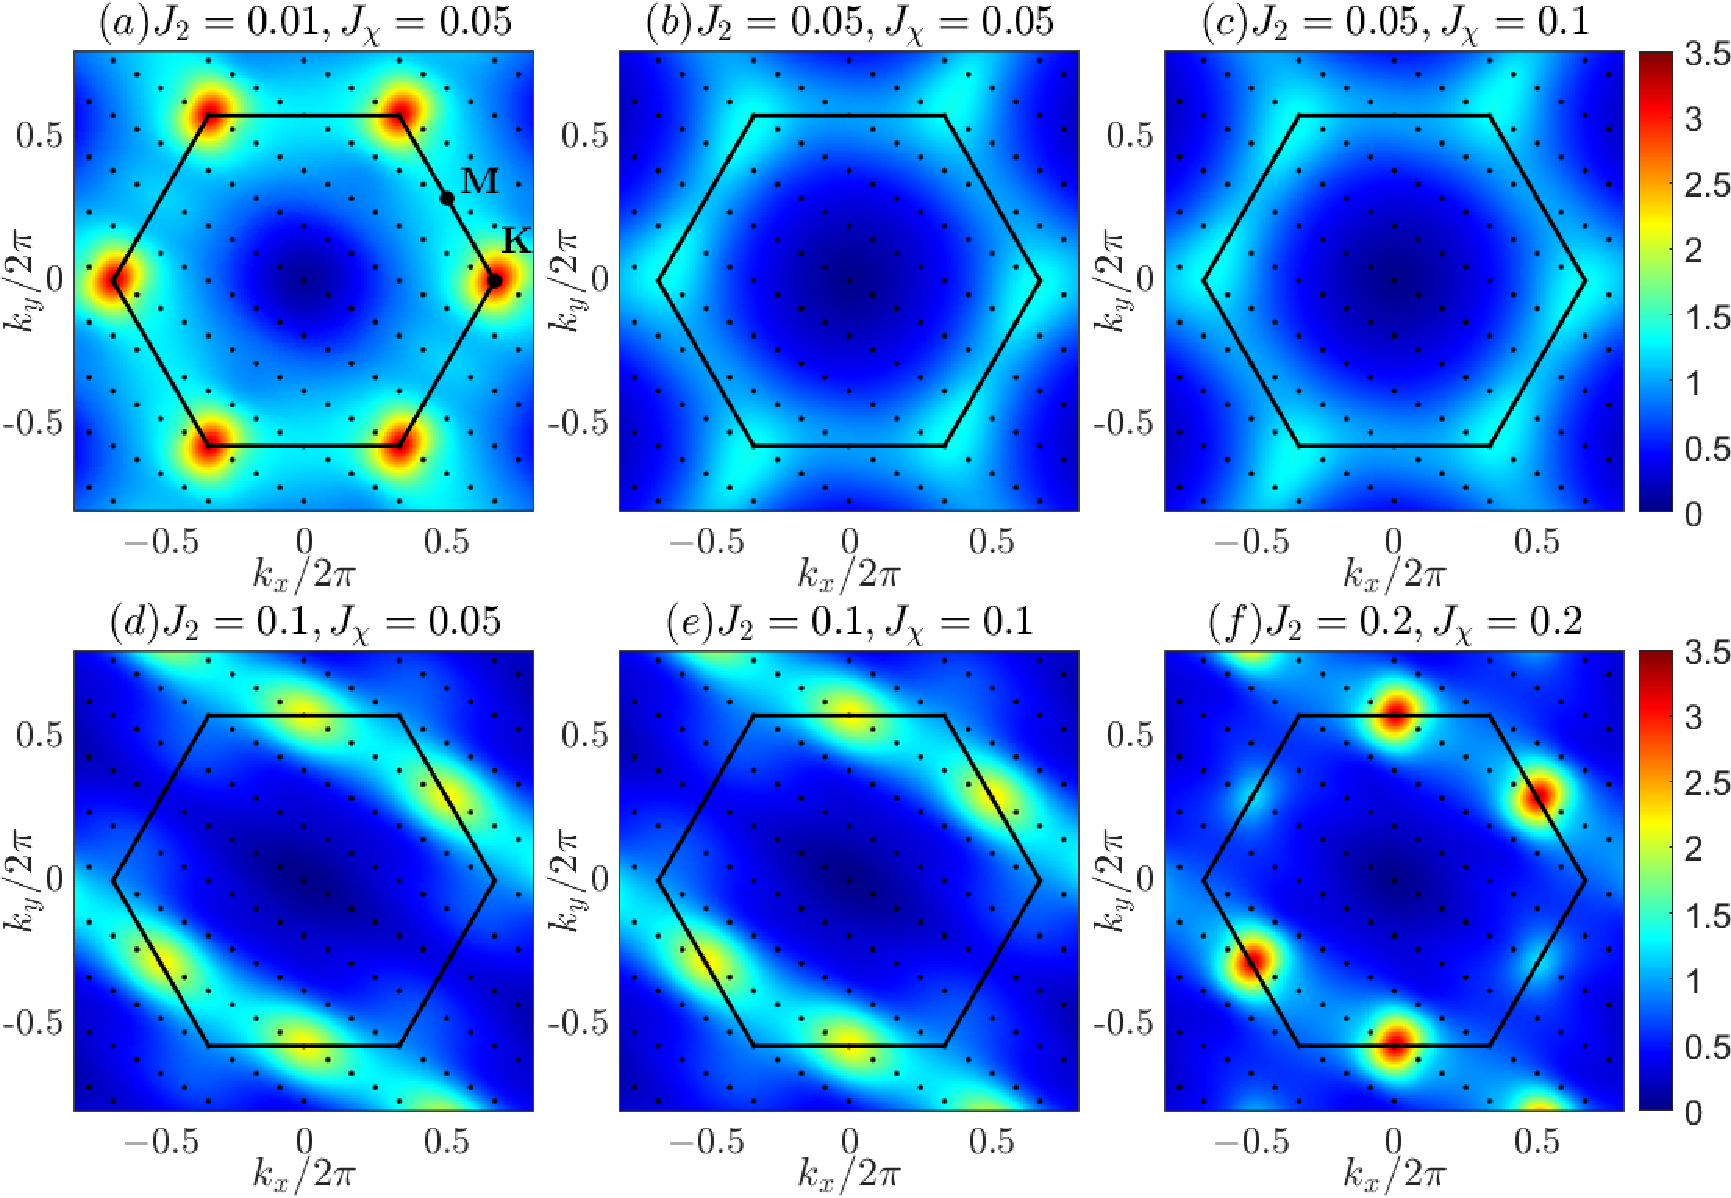
\includegraphics[width=1\linewidth]{Spin_structure_new.pdf}
\caption{The spin structure factor $S(\mathbf{k})$ obtained on $N=36\times 6$ cylinder using correlations from middle $N'=12\times 6$ sites.  (a) SC1 phase at $J_{2}=0.01$. (b) - (c) isotropic $d+id$-wave TSC phase at $J_{2}=0.05$ with near isotropic structure. (d) - (e) Nematic TSC phase at $J_{2}=0.1$.  (f) SC0 state at $J_{2}=0.2$.  The first Brillouin zone is indicated by the solid line with the $\mathbf{M}$ and $\mathbf{K}$ points marked, and the black dots represent the allowed discrete momenta for the finite system with $12\times 6$ sites. The results are obtained with $M=10000$. The doping level is $\delta=1/12$.}
\label{Fig_spin_structure}
\end{figure}


%%%%%%
\section{Summary and discussion}
\label{summary}
We have extensively studied the ground state of the lightly-doped extended $t$-$J$-$J_{\chi}$ model on the triangular  lattice based on the state-of-the-art DMRG method and   unraveled  a global picture of the emergent unconventional superconductivity in systems with the chiral interactions that could be induced by an external magnetic field~\cite{jiang2020topological}. \oim {We identify three classes of superconducting phases (SC1, SC2, and SC0)  characterized by different topological Chern numbers and pairing symmetries. As next nearest neighbor hopping $t_{2}$ and the related spin coupling $J_{2}$ increase, the critical SC1 state  with  Chern number $C=1$ has a transition to the isotropic TSC
phase, which is a gapped topological $d+id$-wave superconductor with $C=2$. 
 With further increase of $t_{2}$ and $J_{2}$, the  isotropic TSC state has a transition to a nematic TSC state in the smaller $J_{\chi}$ regime, which is an analogy of the nematic fractional quantum Hall state with broken rotational symmetry~\cite{you2014theory,yang2017anisotropic,regnault2017evidence}. A topological phase transition from the $C=2$ TSC states to the nematic d-wave SC0 state with  $C=0$ occurs for larger  $t_{2}$ and $J_{2}$. } The hole dynamics tuned by next nearest neighboring hoppings and spin couplings drives the topological quantum phase transitions between different SC phases, and a small chiral interaction $J_{\chi}\approx 0.01$ stabilizes the SC states.  


The TSC is a long-sought state and  it was conjectured that such a SC state may be realized  by doping a CSL~\cite{kalmeyer1987equivalence, wen1989chiral} if it can win over other competing states varying from a chiral metal~\cite{song2021doping, zhu2022doped} to a fractionalized Wigner crystal~\cite{jiang2017holon,peng2021}. Despite intensive efforts in searching for such  a TSC state in strongly correlated systems  during the past decades, there is only one established example  by unbiased numerical studies  of the  $t$-$J$-$J_{\chi}$ model~\cite{jiang2020topological}. The identified TSC state also showed some  instability on wider cylinder ($L_{y}=6$)~\cite{jiang2020topological} before adding next nearest neighboring hopping, indicating that it is near a phase boundary. \oim{In this work, we uncover a global phase diagram  for  the same  model and unravel  two distinct classes of TSC phases with Chern numbers $C=1,2$, and a nematic d-wave SC phase with $C=0$.} The new insight to the mechanism of the doping induced TSC is that  the TSC can emerge by doping a correlated Mott insulating state with $120^{\circ}$ AFM besides doping a CSL  state. Importantly, the hole dynamics changes the spin background and induces topological quantum phase transition upon doping a magnetic ordered state, widening the opportunity for discovering TSC in triangular compounds. On the other hand, the nematic SC with $C=0$ can emerge from either doping the CSL or magnetic ordered states~\cite{gong2017global}, suggesting  the rich interplay between unconventional SC and spin background.

A recent analytical study~\cite{schrade2021nematic} has identified  topological and nematic SC  in the Moir$\acute{e}$ superlattice of twisted bilayer TMD that realizes effective triangular lattice  model with repulsive interactions. 
While the study addresses the physics in the weak coupling picture with spin-valley fluctuations, it is interesting  to see the  $C=2$ topological $d+id$-wave SC and the nematic d-wave SC being discovered, which may  indicate a possible universal picture for SC on triangular lattice with repulsive interactions. It would be exciting to examine the extended Hubbard model with short-range Coulomb interactions for such systems from weak to strong couplings~\cite{arovas2022hubbard}, which can make further predictions for TMD systems. In light of the theoretical prediction of the $SU(4)$ CSL~\cite{zhang20214} in time-reversal invariant TMD bilayers, we anticipate TSC to be a strong competing state and a rich phase diagram to be revealed. Besides the triangular lattice, it will also be interesting to search for possible TSC states in other systems including  Kagome compounds, where 
Mott insulators show similar rich physics  with emergent CSL~\cite{gong2014}.


%%%%%%
\begin{acknowledgments}
We thank Z. Q. Wang and Yahui Zhang for stimulating discussions. 
This work was supported by  the U.S. Department of Energy, Office of Basic Energy Sciences under Grant No. DE-FG02-06ER46305. 
\end{acknowledgments}

%%%%%%%%
\textit{Data availability.---}
Data and simulation codes are available from the corresponding author upon reasonable request.

%%%%%%

%References%%%%%%%%%%%%%%%%%%%%%%%%%%%%%%%%%%%%%%%%

\bibliography{Tr_tJJchi}

% Create the reference section using BibTeX:
%\bibliography{}

%%%%%%%%%%%%%%%%%%%%%%%%%%%%%%%%%%%%%%%%%%%%%%%%%%%


\end{document}